% -*- TeX -*- -*- UK -*- -*- BMR -*-
% ----------------------------------------------------------------
% Beamer presentation ************************************************
%
% Subhaneil Lahiri's template
%
% To compile:
%   Ctrl-Shift-P
%
% **** -----------------------------------------------------------
\documentclass{beamer}
\usetheme{Madrid}

%---------Packages-------------------------------------------------------

% For double screen:
%\usepackage{pgfpages}
%\setbeameroption{show notes on second screen=right}
%
% For finding documentation:
%\usepackage[centertags]{amsmath}
%\usepackage{amssymb}
%\usepackage{xcolor}
\usepackage{pgf}
%\usepackage{graphicx}
%\usepackage{graphics}
%
%\usepackage{ifpdf}
\ifpdf
\else
\DeclareGraphicsRule{.png}{eps}{.bb}{}
\fi
%\usepackage{beamerprosper}
\usepackage{multimedia}

%---------Colours---------------------------------------------------------

% \newrgbcolor{LemonChiffon}{1. 0.98 0.8}
% \newrgbcolor{myellow}{.9 .8 .1}
% \newrgbcolor{myblue}{.2 .36 .77}
% \newrgbcolor{orange}{0.8 0.7 0.2}
% \newrgbcolor{myred}{0.95 0.0 0.0}
\definecolor{darkgrey}{rgb}{.5 .5 .5}
\definecolor{darkblue}{rgb}{0.27843137 0.27058824 0.5372549}
\definecolor{darkred}{rgb}{0.5372549 0.27843137 0.27058824}

%---------Commands-------------------------------------------------------

\newcommand{\rref}[1]{\hfill \small{\color{darkgrey} [#1]}}
\newcommand{\rrref}[1]{ {\color{darkgrey} #1}}

\input{mydefs.tex}
\input{slidesymb.tex}



%---------Title-----------------------------------------------------------

\title{Eigen-larvae}
%
%\subtitle{\small{based on \texttt{arXiv: [hep-th]} with }}
%
\author{Subhaneil Lahiri}
%
\institute[Harvard]{%
Harvard University
}
%
%\slideCaption{}

%---------Beginning--------------------------------------------------------

\begin{document}

%%-------------Slide--------------------------------------------------------
%
%\begin{frame}
%%
% \titlepage
%%
%\end{frame}

%%-------------Slide--------------------------------------------------------
%
%\begin{frame}{Outline}
%%
% \tableofcontents
%%
%\end{frame}

\section{Headsweeps}

%-------------Slide--------------------------------------------------------

\begin{frame}{Rejected headsweep}
%
 \begin{center}
 % divide width/height by 4.
 \movie[width=160px,height=120px,showcontrols=true,loop,poster]{}{hsr.avi}
 \end{center}
%
\end{frame}

%-------------Slide--------------------------------------------------------
\begin{frame}{Accepted headsweep}
%
 \begin{center}
 % divide width/height by 4.
 \movie[width=160px,height=120px,showcontrols=true,loop,poster]{}{hsa.avi}
 \end{center}
%
\end{frame}

%-------------Slide--------------------------------------------------------

\begin{frame}{Eigen-worms}
%
\begin{tabular}{ll}
   \parbox{7.5cm}{\input{worm.TpX}}
   \parbox{4cm}{$s=$ fractional distance along centre-line.\\[0.5cm]
    Parameterise posture as $\theta(s)-\int\theta(s')\dr s'$\\[0.5cm]
    PCA $\implies$ 4 modes.}
 \end{tabular}

 \rref{Stephens et al.}
%
\end{frame}

%-------------Slide--------------------------------------------------------

\begin{frame}{Eigen-larvae?}
%
\begin{tabular}{ll}
   \parbox{7.5cm}{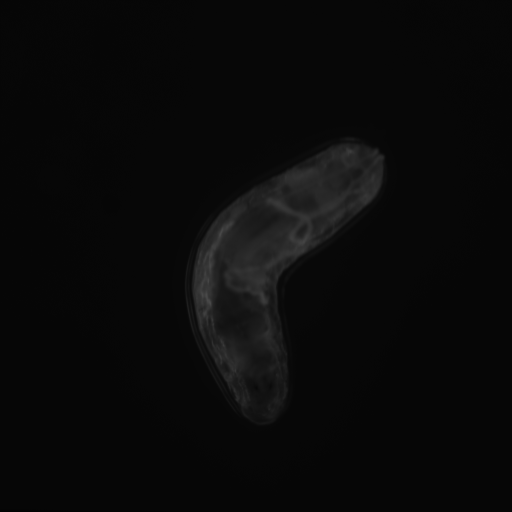
\includegraphics[width=74.60mm]{larva}}
   \parbox{4cm}{Posture not captured by centre-line.\\[0.5cm]
    Length is dynamical.}
 \end{tabular}

%
\end{frame}


\section{Principal Component Analysis}

%-------------Slide--------------------------------------------------------

\begin{frame}{Principal Component Analysis (PCA)}
%
 Our data-set consists of vectors (each member from one frame of the videos):
 %
 \begin{equation*}
   \mathbf{x}_1,\mathbf{x}_2,\mathbf{x}_3,\ldots
 \end{equation*}
 %
 Make change of variables (describe each frame by $\alpha^n$):
 %
 \begin{equation*}
   \mathbf{x}_i = \av{\mathbf{x}} + \sum_n \alpha^n_i \mathbf{u}_n.
 \end{equation*}
 %
 Choose directions $\mathbf{u}_n$ to be of decreasing importance so we can ignore all but first few $\alpha^n$.
%
\end{frame}

%-------------Slide--------------------------------------------------------

\begin{frame}{Principal Component Analysis (cont'd)}
%
 \begin{itemize}
   \item Choose direction $\mathbf{u}_1$ to account for the maximum variance possible.
   \item Choose direction $\mathbf{u}_2$ to account for as much of the remaining variance as possible.
   \item And so on.
 \end{itemize}

 $\implies$ $\mathbf{u}_n$ are eigenvectors of the covariance matrix:
 %
 \begin{equation*}
   \mathbf{C} = \av{ (\mathbf{x}-\av{\mathbf{x}})\cdt(\mathbf{x}-\av{\mathbf{x}})^\mathrm{T} },
   \qquad
   \mathbf{C} \cdt \mathbf{u}_n = \sigma^2_n \mathbf{u}_n.
 \end{equation*}
 %
 where $\sigma^2_n$ are decreasing -- variance accounted for by $n^{th}$ direction.
%
\end{frame}

%-------------Slide--------------------------------------------------------

\begin{frame}{PCA with constraints}
%
 Suppose each datum satisfies a \alert{linear} constraint:
 %
 \begin{equation*}
   \mathbf{b}\cdt \mathbf{x}_i = \beta.
 \end{equation*}
 %
 We have
 %
 \begin{equation*}
 \begin{aligned}
   \mathbf{b}\cdt \av{\mathbf{x}} &= \beta, \\
   \mathbf{b}\cdt \mathbf{C} &= 0 \qquad \implies
   \mathbf{b}\cdt \mathbf{u}_n = 0 
   \quad\text{if}\quad \sigma^2_n \neq 0.
 \end{aligned}
 \end{equation*}
 %
 So, if we choose $\alpha^n=0$ in null directions:
 %
 \begin{equation*}
   \mathbf{b}\cdt \brk{ \av{\mathbf{x}} + \sum_n \alpha^n \mathbf{u}_n } = \beta.
 \end{equation*}
 %
 \ie the constraint is satisfied for any choice of $\{\alpha^n\}$ in non-null directions.
%
\end{frame}

\section{Extracting data}

%-------------Slide--------------------------------------------------------

\begin{frame}{Analysing larva image}
%
\begin{tabular}{ll}
   \parbox{7.5cm}{\input{larvadata.TpX}}
   \parbox{4cm}{\begin{enumerate}
                  \item<1-> Extract boundary
                  \item<2-> Find tail
                  \item<3-> Mark $N$ points along boundary
                  \item<4-> Record difference vectors
                  \item<5-> Rotate so that tangent horizontal at tail
                \end{enumerate}}
 \end{tabular}
%
\end{frame}

%-------------Slide--------------------------------------------------------

\begin{frame}{Parameterising posture}
%
 We record:
 %
 \begin{equation*}
   \mathbf{x} = (\Delta x_1,\ldots,\Delta x_N,\Delta y_1,\ldots,\Delta y_N)^\mathrm{T}
 \end{equation*}
 %
 Constraints:
 \begin{itemize}
 \item $\sum_n \Delta x_n = 0$
 \item $\sum_n \Delta y_n = 0$ (closed curve)
 \item$\Delta y_1 + \Delta y_N = 0.$ (overall rotations)
 \end{itemize}

 \vp All linear $\implies$ respected by PCA.
%
\end{frame}


\section{Results}

%-------------Slide--------------------------------------------------------

\begin{frame}{Dimensionality reduction}
%
 \begin{center}
   \input{stair.TpX}
 \end{center}

 \cf for C.elegans, 95\% of variance from 4 eigen-worms.
%
\end{frame}

%-------------Slide--------------------------------------------------------

\begin{frame}{Dimensionality reduction}
%
 \begin{center}
   \input{bar.TpX}
 \end{center}
%
\end{frame}

%-------------Slide--------------------------------------------------------

\begin{frame}{Eigen-larvae}
%
 \begin{center}
   \input{emags.TpX}
 \end{center}

%
\end{frame}

%-------------Slide--------------------------------------------------------

\begin{frame}{Trajectories for accepted headsweeps}
%
 \begin{center}
   \input{trajectories.TpX}
 \end{center}

%
\end{frame}

% Press Ctrl-D to insert a new slide

%-----End----------------------------------------------------------------

\end{document}
